
\documentclass[a4paper,UKenglish,cleveref, autoref, thm-restate]{lipics-v2021}
%This is a template for producing LIPIcs articles. 
%See lipics-v2021-authors-guidelines.pdf for further information.
%for A4 paper format use option "a4paper", for US-letter use option "letterpaper"
%for british hyphenation rules use option "UKenglish", for american hyphenation rules use option "USenglish"
%for section-numbered lemmas etc., use "numberwithinsect"
%for enabling cleveref support, use "cleveref"
%for enabling autoref support, use "autoref"
%for anonymousing the authors (e.g. for double-blind review), add "anonymous"
%for enabling thm-restate support, use "thm-restate"
%for enabling a two-column layout for the author/affilation part (only applicable for > 6 authors), use "authorcolumns"
%for producing a PDF according the PDF/A standard, add "pdfa"

%\pdfoutput=1 %uncomment to ensure pdflatex processing (mandatatory e.g. to submit to arXiv)
%\hideLIPIcs  %uncomment to remove references to LIPIcs series (logo, DOI, ...), e.g. when preparing a pre-final version to be uploaded to arXiv or another public repository

%\graphicspath{{./graphics/}}%helpful if your graphic files are in another directory

\bibliographystyle{plainurl}% the mandatory bibstyle

% fast and exact
\title{Combining Predicted and Live-Traffic with Time-Dependent A* Potentials} %TODO Please add

%\titlerunning{Dummy short title} %TODO optional, please use if title is longer than one line

% \author{Jane {Open Access}}{Dummy University Computing Laboratory, [optional: Address], Country \and My second affiliation, Country \and \url{http://www.myhomepage.edu} }{johnqpublic@dummyuni.org}{https://orcid.org/0000-0002-1825-0097}{(Optional) author-specific funding acknowledgements}%TODO mandatory, please use full name; only 1 author per \author macro; first two parameters are mandatory, other parameters can be empty. Please provide at least the name of the affiliation and the country. The full address is optional. Use additional curly braces to indicate the correct name splitting when the last name consists of multiple name parts.

\author{Nils Werner}{Karlsruhe Institute of Technology, Germany}{}{}{}
\author{Tim Zeitz}{Karlsruhe Institute of Technology, Germany}{tim.zeitz@kit.edu}{https://orcid.org/0000-0003-4746-3582}{}

\authorrunning{N. Werner and T. Zeitz} %TODO mandatory. First: Use abbreviated first/middle names. Second (only in severe cases): Use first author plus 'et al.'

\Copyright{Nils Werner and Tim Zeitz} %TODO mandatory, please use full first names. LIPIcs license is "CC-BY";  http://creativecommons.org/licenses/by/3.0/

% \ccsdesc[100]{\textcolor{red}{Replace ccsdesc macro with valid one}} %TODO mandatory: Please choose ACM 2012 classifications from https://dl.acm.org/ccs/ccs_flat.cfm
\ccsdesc[500]{Theory of computation~Shortest paths}
\ccsdesc[300]{Mathematics of computing~Graph algorithms}
\ccsdesc[500]{Applied computing~Transportation}

\keywords{realistic road networks, route planning, shortest paths, traffic-aware routing, live traffic} %TODO mandatory; please add comma-separated list of keywords

% \category{} %optional, e.g. invited paper

% \relatedversion{} %optional, e.g. full version hosted on arXiv, HAL, or other respository/website
%\relatedversiondetails[linktext={opt. text shown instead of the URL}, cite=DBLP:books/mk/GrayR93]{Classification (e.g. Full Version, Extended Version, Previous Version}{URL to related version} %linktext and cite are optional

%\supplement{}%optional, e.g. related research data, source code, ... hosted on a repository like zenodo, figshare, GitHub, ...
%\supplementdetails[linktext={opt. text shown instead of the URL}, cite=DBLP:books/mk/GrayR93, subcategory={Description, Subcategory}, swhid={Software Heritage Identifier}]{General Classification (e.g. Software, Dataset, Model, ...)}{URL to related version} %linktext, cite, and subcategory are optional

%\funding{(Optional) general funding statement \dots}%optional, to capture a funding statement, which applies to all authors. Please enter author specific funding statements as fifth argument of the \author macro.

\acknowledgements{I want to thank \dots}%optional

%\nolinenumbers %uncomment to disable line numbering



%Editor-only macros:: begin (do not touch as author)%%%%%%%%%%%%%%%%%%%%%%%%%%%%%%%%%%
\EventEditors{John Q. Open and Joan R. Access}
\EventNoEds{2}
\EventLongTitle{42nd Conference on Very Important Topics (CVIT 2016)}
\EventShortTitle{CVIT 2016}
\EventAcronym{CVIT}
\EventYear{2016}
\EventDate{December 24--27, 2016}
\EventLocation{Little Whinging, United Kingdom}
\EventLogo{}
\SeriesVolume{42}
\ArticleNo{23}
%%%%%%%%%%%%%%%%%%%%%%%%%%%%%%%%%%%%%%%%%%%%%%%%%%%%%%

\newcommand*{\pred}{p}
\newcommand*{\comb}{c}
\newcommand*{\opttt}{\mathcal{T}}
\newcommand*{\dist}{\mathcal{D}}
\newcommand*{\lb}{\mathcal{L}}

\newcommand*{\tdep}{\tau^{\operatorname{dep}}}
\newcommand*{\tmax}{\tau^{\max}}

\newcommand*{\gchu}{G^{\uparrow}}
\newcommand*{\gchd}{\overleftarrow{G^{\downarrow}}}

\usepackage[algo2e,vlined]{algorithm2e}
\usepackage{booktabs}

\begin{document}

\maketitle

%TODO mandatory: add short abstract of the document
\begin{abstract}
Lorem ipsum dolor sit amet, consectetur adipiscing elit. Praesent convallis orci arcu, eu mollis dolor. Aliquam eleifend suscipit lacinia. Maecenas quam mi, porta ut lacinia sed, convallis ac dui. Lorem ipsum dolor sit amet, consectetur adipiscing elit. Suspendisse potenti. 
\end{abstract}

\newpage

\section{Introduction}

An important feature of modern routing applications and navigation devices is the integration of traffic information into routing decisions.
The more comprehensive the considered traffic information, the better the suggested routes, the more accurate the predicted arrival times and ultimately, the more satisfied the users.
For routing, we can distinguish between two aspects of traffic:
On the one hand, there are \emph{predictable} traffic flows.
For example certain highways will consistently have traffic jams on weekday afternoons due to commuters driving home.
On the other hand, unexpected events such as accidents may also have significant influence on the \emph{current} traffic situation.
While it may be sufficient to focus on the current traffic situation to answer short-range routing request, mid- and long-range queries require taking both types of traffic into account.
% example with traffic jam now and in 300km?
We therefore aim to provide routing algorithms which incorporate \emph{combined} predicted and live traffic information.

A common approach for routing in road networks is to model the network as a directed graph where intersections become vertices and road segments become edges.
With edge weights representing travel times, routing requests can be answered by solving the classical shortest path problem.
When considering predicted traffic, edge weights can be modeled as functions of the daytime, which is commonly referred to as \emph{time-dependent routing}.
Dijkstra's algorithm can be used to solve these problems exactly and, at least from a theoretical perspective, efficiently~\cite{d-ntpcg-59}.
However, on the continental-sized road networks used in modern routing applications, it may take seconds to answer mid- or long-range queries which is too slow for most practical applications.
We therefore study algorithms to compute shortest paths significantly faster than Dijkstra's algorithm while retaining exactness.

In this work, we utilize the A* algorithm~\cite{hnr-afbhd-68} for this.
A* can be seen as an extension of Dijkstra's algorithm.
Dijkstra's algorithm explores all vertices closer to the origin than the destination by utilizing a queue where vertices are ordered by their distance from the origin vertex.
A* changes the order in which vertices are visited by adding an estimate of the remaining distance to the queue key, sometimes called \emph{heuristic} or \emph{potential}.
The performance depends on the tightness of these estimates.
The algorithmic core idea of this work are time-dependent potential functions, i.e.\ we obtain tighter estimates by taking the time a vertex is visited into account.

\subsection{Related Work}

Efficient and exact route planning in road networks has received a significant amount of research effort in the past decade.
Since a comprehensive overview is beyond the scope of this paper, we refer to~\cite{bdgmpsww-rptn-16} for an overview.
An approach that has proven quite effective is to exploit that road networks rarely change and usually many queries have to be answered on the same network.
Thus, these queries can be accelerated by computing auxiliary data in an off-line preprocessing phase.

A popular technique following this approach is \emph{Contraction Hierarchies} (CH)~\cite{gssv-erlrn-12}.
During the preprocessing vertices are heuristically ranked by importance (more important vertices are part of more shortest paths).
Shortcut edges are inserted to skip over unimportant vertices.
This allows for a very fast query where only few vertices are explored.
On typical continental-sized benchmark instances, queries take well below a millisecond.
\emph{Multi-Level Dijkstra} (MLD)~\cite{swz-umlgt-02} is a similar approach which also utilizes shortcut edges but inserts them based on a multi-level partitioning.
It achieves slightly slower query times around a millisecond.
MLD is popular for being the first algorithm to support the concept of \emph{customizability} and therefore sometimes also referred by \emph{Customizable Route Planning} (CRP)~\cite{dgpw-crprn-13}.
The \emph{customization} is a second faster preprocessing phase which allows integrating arbitrary weight functions (or live-traffic updates the current weights) into the auxiliary data without rerunning the whole slow first preprocessing phase.
The MLD customization takes a couple of seconds which allows running it every minute.
CH was later generalized to support customizability as well which resulted in Customizable Contraction Hierarchies (CCH)~\cite{dsw-cch-15}.

Both CH and MLD have been extended to time-dependent routing.
However, dealing with weight functions instead of scalar weights makes the preprocessing much harder and leads to difficult trade-offs.
TCH~\cite{bgsv-mtdtt-13} has fast queries but a very expensive preprocessing phase (may take hours) and may produce prohibitive amounts of auxiliary data (> 100\,GB).
% TODO 3-phase not introduced
TD-CRP~\cite{bdpw-dtdrp-16} (the MLD variant) still follows a 3-phase approach and has a relatively fast customization phase.
However, this is only possible by giving up exactness.
Also, TD-CRP does not support path unpacking.
CATCHUp~\cite{swz-sfert-21} adapts CCH to the time-dependent setting and has fast and exact queries with significantly reduced memory consumption.
While it has a customization phase, running it takes significantly longer than a traditional CCH or CRP customization.
On the benchmark graphs used in this paper, a CATCHUp customization may even take hours, which is too slow for a live-traffic updates setting.
% TDS?, (Shark?)

A* has also been utilized in speed-up techniques for routing in road networks.
With ALT~\cite{gh-cspas-05,gw-cppsp-05}, a few landmark vertices are selected during preprocessing.
From and to these vertices distances to all other vertices are precomputed.
During queries, these distances are combined with the triangle inequality to obtain distance estimates to the target vertex.
ALT is quite popular and has also received research interest in areas beyond route planning.
However, query times are significantly slower than with shortcut-based approaches such as CH or MLD.
ALT has also been extended to dynamic and time-dependent settings~\cite{dn-crdtd-12}. % combined?
However, the model studied there is not as general as with customization based approaches.
% Core-ALT?
Another more recent A*-based approach is CH-Potentials~\cite{strasser_et_al:LIPIcs.SEA.2021.6}.
As the name suggests, CH-Potentials extract distance estimates from a CH which leads to tighter estimates and faster queries than with ALT.
For this, the Lazy RPHAST algorithm is introduced which we also heavily use in this work.
CH-Potentials can be applied to a variety of routing problem variants and the original publication even mentions a combination of live and predicted traffic.
However the reported query times are a above 100\,ms which we consider too slow for practical applications.

\subsection{Contribution}

In this work, we introduce a time-dependent generalization of A* potentials.
We then propose two efficient algorithms for such time-dependent A* potentials and discuss how to apply them to efficiently answer queries in a combined live and predicted traffic setting.
An extensive evaluation confirms the applicability of our algorithms.
Queries incorporating both predicted and the current traffic can usually be answered within few tenths of milliseconds.
Live-traffic updates can be integrated within less than a minute.
Compared to Dijkstra's algorithm, we achieve a speed-up of around two orders of magnitude and compared to a time-independent CH-Potential, we achieve a speed-up of up to an order of magnitude.
% Introduce A* with TDPot
% Introduce 2 TDPots
% Show how to apply them to live traffic
% Extensive eval
% up to one order of mag over time independent pot
% 2 orders of magnitude over dijkstra

\section{Preliminaries}
We consider directed graphs $G=(V,E)$ with $n=|V|$ vertices and $m=|E|$ edges.
We use $uv$ as a short notation for an edge from a \emph{tail} vertex $u$ to \emph{head} vertex $v$.
Weight function $w : E \to (\mathbb{Z} \to \mathbb{Z}^{\geq 0})$ map edges to time-dependent functions.
These functions map a departure $\tau$ at the tail $u$ to a travel time $w(uv)(\tau)$.
The arrival at the head $v$ is thus $w(uv)(\tau) + \tau$.
To simplify notation we will often write $w(uv, \tau)$.
Further, when it is clear from context that we talk about constant travel time functions, we will omit the time argument and write $w(uv)$.
We extend the weight function definition to paths:
The travel time of a path $P = (v_1,\dots,v_k)$ can be obtained by successively evaluating the edges travel times: $w(P, \tau) = w(v_1 v_2, \tau) + w_((v_2,\dots,v_k), \tau + w_{v_1 v_2}(\tau))$.
We assume that all travel time functions adhere to the \emph{first-in first-out} (FIFO) property, i.e.\ departing later may never lead to an earlier arrival.
Formally stated this means $\tau + w(\tau) \leq \tau + \epsilon + w(\tau + \epsilon)$ for any $\epsilon \in \mathbb{Z}^{\geq 0}$.
% TODO explain waiting?
With non-FIFO travel time functions, the shortest path problem becomes \textsf{NP}-hard~\cite{or-tnp-89}.

% traffic model
In our problem model, each edge $e \in E$ has a predicted travel time function $\pred(e)$.
Predicted travel time functions are periodic piecewise linear functions represented by a sequence of breakpoints covering one day of predictions.
Further, edges may have a currently observed (constant) live travel time $l(e)$ and a point in time $\tau^{\operatorname{end}}(e)$ when we switch back to the predicted travel time.
We assume that the traffic predictions are a conservative estimate and that live-traffic will always have slower travel times due to accidents and other traffic incidents.
Thus, we define the combined travel time function of an edge as follows:
$\comb(e, \tau) = \max(\pred(e, \tau), \min(l(e), \pred(e, \tau^{\operatorname{end}}(e)) + \tau^{\operatorname{end}}(e) - \tau))$.
% TODO talk about -1 segment
% TODO visualize
% TODO inf

% TODO general td fns vs concrete predicted and combined fns

Our goal is given vertices $s$ and $t$ and an earliest departure $\tdep$ to obtain the path $P = (s,\dots,t)$ that minimizes $\comb(P, \tdep)$.
We refer to the travel time of this path as $\opttt(s,t,\tdep)$.

\subsection{Application Model}

% phases
We consider an application model with three phases.
During the first \emph{preprocessing} phase, the graph topology and traffic predictions are given.
A preprocessing algorithm may use these inputs to precompute auxiliary data which may take several hours.
Preprocessing should still be fast enough to rerun it on a daily basis.
In the second \emph{update} phase, traffic weights are given for the current moment $\tau^{\operatorname{now}}$ and should be incorporated into the precomputed data within as little time as possible.
This phase may be repeated frequently (every few minutes) to adjust to the current state of traffic.
We do not call this phase \emph{customization} because we use customization algorithms from CCH and CATCHUp during both the preprocessing and the update phases.
During the third and final \emph{query} phase, many shortest path queries $(s,t,\tdep)$ where $\tdep \geq \tau^{\operatorname{now}}$ should be answered as quickly as possible.

\subsection{Dijkstra/A*}

% distance vs arrival times
Dijkstra's algorithm computes $\opttt(s,t,\tdep)$ by exploring vertices ordered by increasing distance from $s$ until $t$ is reached.
The distances from $s$ of each vertex $u$ are tracked in an array $\mathtt{D}[u]$, initially set to $\infty$ for all vertices.
A priority queue with vertices ordered by their distance from $s$ is maintained.
The priority queue is initialized with $s$ and $\mathtt{D}[u]$ set to $\tdep$.
In each iteration, the next closest vertex $u$ is extracted from the queue and \emph{settled}.
Outgoing edges $uv$ are \emph{relaxed}, i.e.\ the algorithm checks if $\mathtt{D}[u] + w(uv, \mathtt{D}[u])$ improves $\mathtt{D}[v]$.
If so, the queue position of $v$ is adjusted accordingly.
Once $t$ was settled, the final distance is known and the search can terminate.

% remove?
Dijkstra's algorithm has a worst case running time of $\mathcal{O}((n + m) \log n)$ when the queue is implemented as a $k$-ary heap.
In the presence of negative edge weights, Dijkstra still will find correct shortest distances, as long as there are no negative cycles.
However, distances may not be final anymore after a vertex was settled.
The algorithm is then denoted as \emph{label-correcting} instead of \emph{label-setting}.

% search space
% heurisitc vs potential
A* is an extension of Dijkstra's algorithm where the search is guided towards the target through a potential function $\pi_t$ which estimates the remaining distance to the target.
This estimate is added to the queue key.
Thus, vertices closer to the target a visited earlier and the search space becomes smaller.
In this paper, we propose time-dependent potentials $\pi_t : V \to (T \to \mathbb{Z}^{\geq 0})$.
By mapping each vertex to a time-dependent function, we can obtain tighter estimates and accelerate queries further.
Analogue to classical potentials, there are several important properties when discussing the correctness of potential functions:
\begin{itemize}
  \item Feasibility: $w_(uv, \tau) + \pi_t(v, \tau + w(uv, \tau)) - \pi_t(u, \tau) \geq 0$ for all edges $uv \in E$ and times $\tau$
  \item Lower bound: $\pi_t(v, \tau) \leq \dist(v,t,\tau)$ for all vertices $v \in V$ and times $\tau$
  \item First-In First-Out (FIFO): $\pi_t(v, \tau) \leq \pi_t(v, \tau + \epsilon) + \epsilon$ for all vertices $v \in V$, times $\tau$ and $\epsilon \geq 0$
\end{itemize}
The FIFO property must hold for all time-dependent potentials for A* to work properly.
For feasible potentials, A* is label-setting and a running time of $\mathcal{O}((n + m) \log n)$ is guaranteed.
With lower-bound potentials, A* may be label-correcting but will have determined the shortest distance once $t$ is settled for the \emph{first} time.
To answer a concrete query $s,t,\tdep$ it is actually sufficient to fulfill these properties only for very specific instants, i.e.\ for $\tau = \dist(s,u, \tdep)$ the best possible arrival at each vertex $u$.
Our proposed potentials heavily rely on this and only compute potential data for the specific moments necessary to answer a query correctly.
In Appendix~\ref{sec:correctness} we derive and discuss the correctness properties in detail, formally prove that queries will be answered correctly with these properties and also give proofs for the potentials proposed in the next section.

% The queue is ordered by $\mathtt{D}[u] + \pi_t(u)$.
% A* is equivalent to running Dijkstra's algorithm on a graph with modified weights $w'_{uv} = w_{uv} + \pi_t(v) - \pi_t(u)$.
% If this modified weight is non-negative for all weights, a potential function is called \emph{feasible}.
% For feasible potentials, A* has the same theoretical worst-case running time as Dijkstra's algorithm and will always have obtained the optimal distance once $t$ was settled.
% A* will also obtain correct results when $\pi_t(v) \leq \dist(v, t)$ for all vertices $v \in V$. % TODO proof
% Even when the modified weights may have negative weights, all vertices on the shortest path will have a queue key smaller than the target.
% Thus, we can prove inductively, that the shortest path and distance will have been found, once $t$ is settled.
% Nevertheless, the label-setting property is not given anymore and vertices other than $t$ may be settled multiple time.
% The theoretical worst-case running time can also not be guaranteed anymore.

% We now generalize the notion of potentials to the time-dependent setting and propose \emph{time-dependent potentials}.
% % TODO time domain
% A time-dependent potential maps a vertex to a time-dependent function $\pi_t : V \to (T \to \mathbb{Z}^{\geq 0})$.
% The function maps instant to an estimate of the remaining travel time to the target.



\subsection{Contraction Hierarchies}

\emph{Contraction Hierarchies} (CH) is a speed-up technique to accelerate shortest path computations on road networks through precomputation.
For a detailed discussion we refer to~\cite{gssv-erlrn-12}.
% Here, we briefly introduce necessary notation and concepts used in this paper.
During the preprocessing, vertices are ordered totally by ``importance'' where more important vertices should lie on more shortest paths.
Intuitively, vertices on highways are more important than vertices on rural streets.
Then, an \emph{augmented graph} $G^+$ with additional \emph{shortcut edges} is constructed.
Shortcut edges are inserted in such a way that between any two vertices $s$ and $t$ there exists a path of shortest distance which uses no vertices less important than $s$ and $t$.
This allows finding shortest paths by running Dijkstra's algorithm from both $s$ and $t$ and only following edges toward more important vertices.
Formally, we split $G^+$ into $\gchu$ and $G^{\downarrow}$ where $\gchu$ only contains arcs $uv$ where $u$ is less important than $v$ and $G^{\downarrow}$ vice versa and run Dijkstra's algorithm from $s$ on $\gchu$ and from $t$ on $\gchd$.

In this work we build on \emph{Customizable Contraction Hierarchies} (CCH)~\cite{dsw-cch-15}.
For CCH, the construction of the augmented graph is split in three stages.
First, the vertex ordering is obtained using nested dissection.
A balanced vertex separator is computed heuristically and the vertices in it are assigned the highest importance.
The process is then recursively applied to all cells.
In the second stage the topology of the augmented graph is computed.
For this, vertices are processed by ascending importance.
For every vertex, its neighborhood of more important vertices is completed to form a clique.

In the final stage, the \emph{customization}, the weights of the augmented graph are computed.
The first step of the customization is to apply the current weights to the respective edge weights in the augmented graph.
All other edges in the augmented graph are set to $\infty$.
In the second step, the algorithm iterates over all edges $uv$ ordered increasingly by the ranks of the endpoints.
For each edge, all \emph{lower triangles} $(u,w,v)$ where both $uw$ and $wv \in E^+$ and $w$ has a smaller importance than both $u$ and $v$ are enumerated and relaxed, i.e.\ if $w(uv)$ is set to $\min(w(uv), w((u,w,v)))$.
Now, each edge has the weight of the shortest path using only lower ranked vertices which is sufficient to allow applying the CH query algorithm.
% basic customization
However, not all of these edges are necessary.
In an optional further step, the \emph{perfect customization}, unnecessary edges are identified.
For this, all edges are processed again but this time in a top-down fashion, i.e\ ordered decreasingly by the ranks of the endpoints.
Now, for each edge, all \emph{intermediate triangles} and \emph{upper triangles} $(u,w,v)$ where both $uw$ and $wv \in E^+$ and $w$ has a smaller importance than either $u$ and $v$ are enumerated and relaxed, i.e.\ if $w(uv)$ is set to $\min(w(uv), w((u,w,v)))$.
Now, each edge in the augmented graph has the weight of the shortest distance between its endpoints.
The authors of~\cite{dsw-cch-15} proved that only edges for which the weight remained unchanged during the perfect customization are necessary to guarantee the correctness of the CH query algorithm.
Thus, in a final step all edges with changed weights are removed and a \emph{reduced augmented graph} is constructed.
% perfect not always necessary

CATCHUp~\cite{swz-sfert-21} is a time-dependent adaption of CCH.
In this paper, we utilize its preprocessing as a block box.
This gives us for each edge in the augmented a relatively tight lower bound approximation of the shortest path through lower ranked nodes, i.e.\ the result of a time-dependent basic customization.
Further, we get tighter scalar lower and upper bounds than we would get by applying the classical customization algorithms on constant upper and lower bound weight functions.
CATCHUp does not support a time-dependent perfect customization.
However, a decent number of edges can still be removed by utilizing the scalar bounds.
For this, the perfect customization is run on scalar upper bounds.
Then for each bound the lower bound (which is valid for the path represented by the shortcut) can be compared to the upper bound (which is a bound on the shortest distance between the endpoints).
Each edge where the shortest path upper bound is smaller then the shortcut lower bound can be removed~\cite{swz-sfert-21}.
We will also utilize this principle for our time-dependent potentials.

\subsection{Lazy RPHAST and CH-Potentials}

Lazy RPHAST~\cite{strasser_et_al:LIPIcs.SEA.2021.6} is a CH-based algorithm to incrementally compute distances from many sources toward a common target
It is a variant of the CH query algorithm where one half of the search is replaced with a recursive depth-first search (DFS) which memoizes distances.
Using a DFS to compute shortest distances works because $\gchu$ is a directed acyclic graph.
The first step is a run Dijkstra's algorithm on $\gchd$ from the target.
Then, the main routing depicted in Algorithm~\ref{algo:lazy_rphast} can be called for every source to obtain the shortest distance to the target.
If the distance of a vertex was previously computed, the routine terminates immediately and returns the memoized value.
Otherwise, the distance is computed as the minimum over the recursively computed distances of the upward neighbors plus the respective edge weights and the distance possibly found in the backward search.
Using Lazy RPHAST as an A* potential is called \emph{CH-Potentials}.
Lazy RPHAST can be applied to CCH without modifications.
% low deg optimizations
% relate to td

\begin{algorithm2e}
\KwData{$\mathtt{D}^{\downarrow}[u]$: tentative distance from $u$ to $t$ computed by Dijkstra's algorithm on $\gchd$}
\KwData{$\mathtt{D}[u]$: memoized final distance from $u$ to $t$, initially $\bot$}
\SetKwFunction{Dist}{ComputeAndMemoizeDist}
\SetKwProg{Fn}{Function}{:}{}
\Fn{\Dist{$u$}}{
    \If{$\mathtt{D}[u] = \bot$}{
        $\mathtt{D}[u]\leftarrow \mathtt{D}^{\downarrow}[u]$\;
        \For{all arcs $uv$ in $\gchu$}{
            $d \leftarrow \Dist(v)$\;
            \If{$\mathtt{D}[u] < d + w(uv)$}{
                $\mathtt{D}[u] \leftarrow d + w(uv)$\;
            }
        }
    }
    \Return{$\mathtt{D}[u]$}\;
}
\caption{Computing the distance from a single vertex $u$ to $t$ with Lazy RPHAST}
\label{algo:lazy_rphast}
\end{algorithm2e}

\section{Algorithms}

\subsection{Multi-Metric Potential}

We now introduce our first time-dependent potential, the \emph{Multi-Metric Potential}.
Let $(s,t,\tdep)$ be a query and $\tmax = \tdep + \opttt(s,t,\tdep)$ the optimal arrival at the target.
Consider any $\tau' \leq \tdep$, $\tau'' \geq \tmax$ and the weight function $l(e) = \min_{\tau' \leq \tau \leq \tau''}\pred_e(\tau)$.
Clearly, $\dist_{l}(v,t)$ provides lower bound estimates of distances to the target vertex during the time relevant for this query.
If $\tau'$ and $\tau''$ are close to $\tdep$ and $\tmax$ and if the difference between $\tau'$ and $\tau''$ is not too big, the estimates will be significantly tighter than global lower bound distances.
The \emph{Multi-Metric Potential} is based on this observation.
Instead of using a single potential based on a global lower bound valid for the entire time, we process multiple lower bound weight functions valid for different time intervals.
At query time, we then select an appropriate weight function.
Efficiently computing distances with respect to the selected weight function is done with the Lazy RPHAST.

\subparagraph{Preprocessing}
The very first step of the preprocessing for this potential is to perform the regular CCH preprocessing, i.e.\ compute a nested dissection order~\cite{ghuw-fbndocch-19} and construct the unweighted chordally completed augmented graph.
Now let $I$ be a set of time intervals.
In our implementation, we use 48 intervals of length 1\,h starting at each full and each half hour, 24 intervals of length 2\,h starting at each full hour, 12 intervals of length 4\,h starting every two hours, 6 intervals of length 8\,h starting every 4 hours, 4 intervals of length 12\,h starting every 6 hours and one interval covering the entire day.
During preprocessing, we extract lower bounds and run the CCH basic customization algorithm for each interval.
This can be trivially parallelized.
Also, the customization can be parallelized internally.
For further engineering details, we refer to~\cite{dsw-cch-15,bsw-rttau-19}.

\subparagraph{Update}
We compute an additional lower bound weight function of length 59\,minutes starting at $\tau^{\operatorname{now}}$ which incorporates the current live traffic situation.
Further, we extract an upper bound weight function for the entire day valid with respect to both the predicted and the live traffic.
We then run both the basic and the perfect customization algorithms for the upper bound without constructing a reduced augmented graph.
Recall that after the perfect customization, each edge in the CCH has the length of the shortest distance between its endpoints.
We now construct a reduced augmented graph for all lower bounds at once.
This graph contains all edges for which the customized global lower bound weight is not greater than the customized upper bound.
Edges where the upper bound now undercuts the global lower bound are removed in \emph{all} lower bound weights.
% could do for each weight seperately but not worth it
Finally, we construct the reduced graph for the upper bound by removing all edges which were improved during its perfect customization.
The running time of the update phase is dominated by the construction of the reduced graphs.
Parallelizing it is crucial to achieve good running times.
See~\cite{bsw-rttau-19} for engineering details.
Note that the graph reduction steps are entirely optional and only serve to optimize query performance.
In case update running times are critical, the graph reduction can be skipped which will slightly worsen the query performance.

\subparagraph{Query}
We perform a classical CCH query on the customized upper bound to obtain a pessimistic estimate of $\tmax$.
We then select the shortest lower bound interval which still fully includes $[\tdep,\tmax]$.
Running Lazy RPHAST on the customized weight function of this interval then yields the potential function.
% Metric switching

% Correctness

\subsection{Interval-Minimum Potential}

The \emph{Interval-Minimum Potential} is a time-dependent adaptation of the Lazy RPHAST algorithm.
Where Lazy RPHAST has a single scalar (lower bound) weight for each edge, the Interval-Minimum Potential has a lower bound function.
This allows for tighter lower bound estimates but introduces new challenges.
First, computing an augmented CH graph with time-dependent travel time functions (even with only approximated lower bound functions) is difficult problem on its own an has been subject to study for entire articles~\cite{bgsv-mtdtt-13,swz-sfert-21}.
We therefore utilize the existing CATCHUp algorithm~\cite{swz-sfert-21}.
Second, storing the travel time functions of an augmented graph can be very expensive in terms of memory consumption.
Also, the usual representation as a list of breakpoints makes the evaluation much more expensive than looking up a scalar weight.
We therefore resort to a different representation and store functions as piecewise constant values in buckets of equal time.
In our implementation, we split the day into 96 buckets of length 15 minutes.
Third, evaluating the lower bound functions requires a time of evaluation.
While we have a time for the vertex for which we compute the potential, Lazy RPHAST also needs a time for every recursive invocation.
We therefore apply Lazy RPHAST a second time on a global upper and lower bound weight function to obtain an arrival interval at each vertex.

\subparagraph{Preprocessing}
The first step is the same as for the Multi-Metric Potential: performing the CCH preprocessing.
Then, we perform a CATACHUp customization.
This yields tight scalar upper and lower bounds as well as time-dependent unpacking information which allows to reconstruct the path represented by a shortcut for each point in time.
The original CATCHUp customization algorithm does not output shortcut travel time functions.
However, approximated functions are maintained throughout the customization.
From these approximated functions, we extract the piecewise constant lower bound buckets for all edges in the augmented graph.

\subparagraph{Update}
As for the Multi-Metric Potential, we extract an upper bound weight function for the entire day valid with respect to both the predicted and the live traffic.
We then run both the basic and the perfect customization algorithms for the upper bound without constructing a reduced augmented graph.
Now, we remove all CCH edges, where the upper bound undercuts the scalar lower bound from the CATCHUp customization and prepare two graphs:
One with the bucket-based time-dependent lower bound functions and another one with the scalar upper and lower bounds.
The running time of this phase is again dominated by the construction of the reduced graphs and the adjustments discussed in the previous section are applicable, too.

% derive from sources when predicted upper bound valid again (this is the reason why not reduced in preprocessing)
% reduced graph bounds
% reduced graph buckets by predicted bounds
% bound switching

\subparagraph{Query}
For the query, we build the potential with two instantiations of the Lazy RPHAST algorithm.
The first one works on the graph with the scalar bounds and computes lower and upper bounds on the distance from the source vertex.
The second one works on the graph with the bucket-based time-dependent lower bound functions.
The second one uses the first one to determine arrival intervals at each vertex which are in turn used to evaluate outgoing edges.

Choosing the right memory layout for the bucket weights is crucial for the performance of this algorithm.
We do store all weights of a single bucket consecutively.
Typically, only few buckets per edge are relevant, because the arrival intervals are relatively tight.
Also, outgoing all edges of each vertex are evaluated consecutively.
Thus, having their weights for the same bucket close to each other increases cache hits.

% evaluation time metric pruning
% correctness

\subsection{Compression}

Both our time-dependent potentials have to store a significant number of weight functions.
This can lead to problematic memory consumption.
However, since we only need lower bounds, we can merge lower bound weight functions into a combined weight function with the respective minimum weights and thus reduce the number of weight functions we need to store.
Thus by trading some lower bound tightness, we can reduce memory consumption.
Dealing with merged lower bound functions can be implemented for both potentials with a layer of indirection which maps each bucket or interval to a weight function id.
Then, when merging to weight functions, we let both buckets/intervals point to the same weight function id.

We now discuss an efficient and well parallelizable algorithm to iteratively merge weight functions until only $k$ functions remain.
In each step, we merge the pair of weight functions with the minimal sum of squared differences over all edge weights.
Since comparing all weight function pairs is expensive, we track the minimum difference sum we have found so far and stop any comparison where the sum exceeds the best sum.
Even when stopping a comparison, we store the sum so far and the edge id up to which we have summed up the differences.
This allows to avoid repeating the work already performed should we need to continue to compare this particular pair of weight functions.
Finally, we maintain all pairs of weights along with the (possibly partial) difference sums in a priority queue ordered by the difference sums.
When merging two weight functions, all other associated queue entries are removed from the queue and new entries for comparisons between the new weight function and all other functions are inserted.
To determine the next weight function pair to merge, unfinished weight function pairs are popped from the queue and processed in parallel.
The minimum difference is tracked in an atomic variable.

\section{Evaluation}
% env
\subparagraph{Environment} Our benchmark machine runs openSUSE Leap 15.3 (kernel 5.3.18), and has 192\,GiB of DDR4-2666 RAM and two Intel Xeon Gold 6144 CPUs, each of which has eight cores clocked at 3.5\,GHz and 8~$\times$~64\,KiB of L1, 8~$\times$~1\,MiB of L2, and 24.75\,MiB of shared L3 cache.
Hyperthreading was disabled and parallel experiments use 16 threads.
We implement our algorithms in Rust\footnote{The code for this paper and all experiments is available at \url{https://github.com/kit-algo/tdpot}} and compile them with \texttt{rustc 1.61.0-nightly (c84f39e6c 2022-03-20)} in the release profile with the \texttt{target-cpu=native} option.
% To compile InertialFlowCutter and RoutingKit which are written in C++, we use GCC~10.3.0 using optimization level 3 and the -march=native option.

\subparagraph{Datasets}
We evaluate our algorithms on two networks where we have proprietary real-world traffic data available.
Sadly, we can not provide access to these datasets due to non-disclosure agreements.
The datasets are the same ones used in~\cite{swz-sfert-21,strasser_et_al:LIPIcs.SEA.2021.6}.
We are not aware of any publicly available traffic feeds or predictions.
%
Our first network, PTV Europe, was provide by PTV\footnote{\url{https://ptvgroup.com}} in 2020 and is based on TomTom\footnote{\url{https://www.tomtom.com}} routing data covering western Europe.
It has 28.5\,M vertices and 61\,M edges.
Three quarters of the edges have a non-constant travel time.
The data includes a traffic incident snapshot from 2020/10/28 07:47 with live speeds and estimated incident durations for 215\,K vertex pairs.
% ignoring too long
%
Our second network, OSM Germany, is derived from an early 2020 snapshot of OpenStreetMap and converted into a routing graph using RoutingKit\footnote{\url{https://github.com/RoutingKit/RoutingKit}}.
The graph has 16.2\,M vertices and 35.2\,M edges.
For this instance, we have proprietary traffic data provided by Mapbox\footnote{\url{https://mapbox.com}}.
This includes traffic predictions for 38\% of the edges as predicted speeds for all five minute periods over the course of a entire week.
We only use the predictions for one day.
Also, we exclude speed values which are faster than the freeflow speed computed by RoutingKit.
The data also includes two live traffic snapshots in the form of OSM node ID pairs and live speeds for the edge between the vertices.
One is from Friday 2019/08/02 15:41 and contains 320\,K vertex pairs and the other from Tuesday 2019/07/16 10:21 and contains 185\,K vertex pairs.
The datasets do no contain any estimate how long the observed live speeds are valid.
We therefore set $\tau_e^{\operatorname{end}}$ to one hour after the snapshot time.
% relative delays?
Note that even though it is smaller and has less time-dependent edges, OSM Germany is actually the harder instance.
This is because it has more breakpoints per time-dependent edge (124.8 compared to 22.5 on PTV Europe) and the predicted travel times fluctuate much stronger.

% {
%   "args": [
%     "target/release/explore_graph_catchup",
%     "/algoDaten/zeitz/roadgraphs/osm_ger_td_build2022/"
%   ],
%   "build_profile": "release",
%   "build_target": "x86_64-unknown-linux-gnu",
%   "build_time": "Wed, 30 Mar 2022 14:56:13 +0000",
%   "build_with_rustc": "rustc 1.61.0-nightly (c84f39e6c 2022-03-20)",
%   "feature_flags": "DEFAULT, TDCCH_APPROX, TDCCH_POSTCUSTOMIZATION, TDCCH_PRECUSTOMIZATION, TDCCH_QUERY_ASTAR, TDCCH_QUERY_CORRIDOR, TDCCH_QUERY_LAZY, TDCCH_TRIANGLE_SORTING",
%   "git_revision": "cebb481",
%   "graph": {
%     "num_arcs": 35186806,
%     "num_constant_ttfs": 21726770,
%     "num_ipps": 1679732710,
%     "num_nodes": 16175148
%   },
%   "hostname": "compute11",
%   "program": "explore_graph_catchup",
%   "relative_delays": {
%     "mean": 0.26955234976571363,
%     "nonconst_mean": 0.8491454402873269,
%     "nonconst_total_relative_delay": 0.788178202531493,
%     "total_relative_delay": 0.0231669950618092
%   },
%   "start_time": "2022-03-30T14:57:42.952792137+00:00",
%   "unprocessed_graph": {
%     "num_arcs": 35186806,
%     "num_ipps": 1679732710,
%     "num_nodes": 16175148
%   }
% }

\subparagraph{Methodology}
We evaluate our algorithms with batches of 100\,K shortest path queries solved sequentially using three different query sets:
First, there are random queries where source and target are drawn from all vertices uniformly at random which leads to mostly long-range queries.
Second are 1h queries where we draw a source vertex uniformly at random, run Dijkstra's algorithm from it and pick the first node with a distance greater one hour as the target.
Third, following the established Dijkstra rank methodology~\cite{}, we generate rank queries for a thorough investigation of the performance by query distance.
For the rank queries, we pick a source uniformly at random and run Dijkstra's algorithm from it.
We use every $2^{i}$th settled vertex as the target of Dijkstra rank $2^i$.
To evaluate the performance of the preprocessing and update phases, we run them 10 and 100 times, respectively.
Preprocessing and update phases utilize all cores using 16 threads.

\begin{figure}
\centering
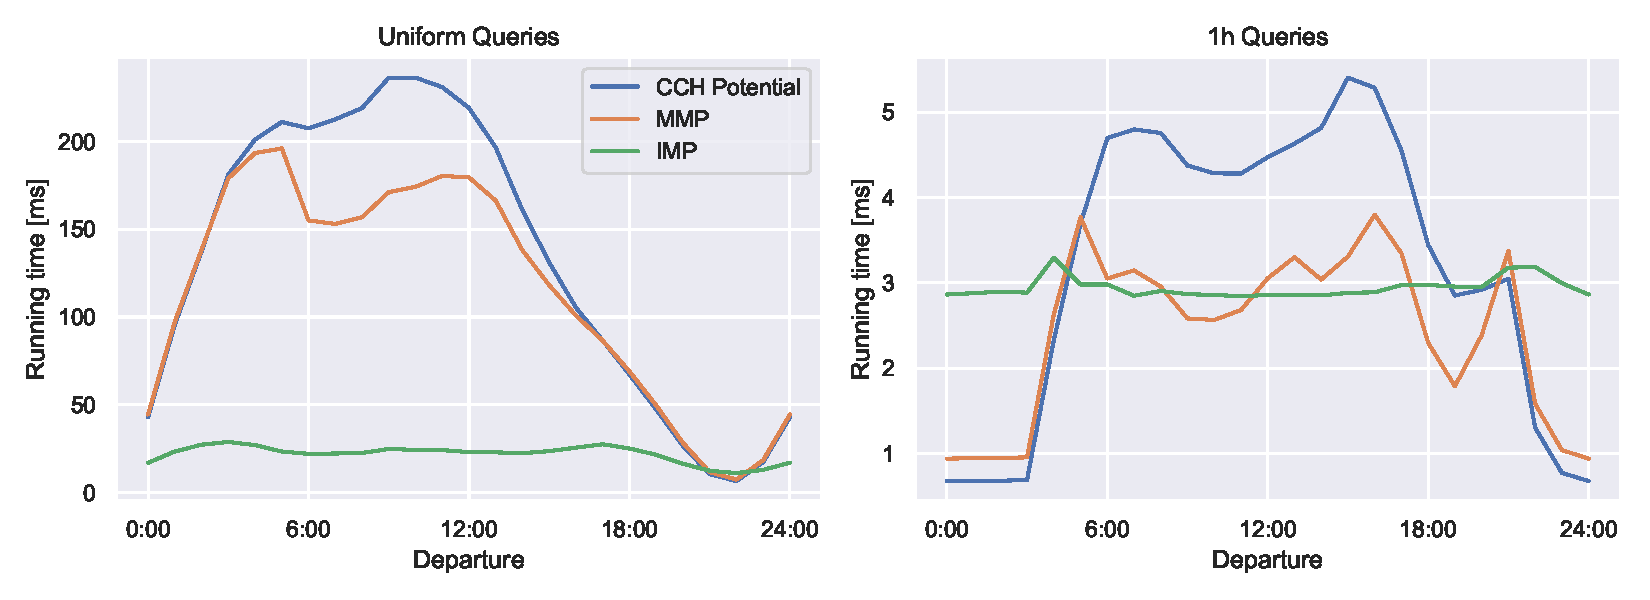
\includegraphics[width=\linewidth]{fig/perf_over_day.pdf}
\caption{
TODO
}\label{fig:by_dep}
\end{figure}

\begin{figure}
\centering
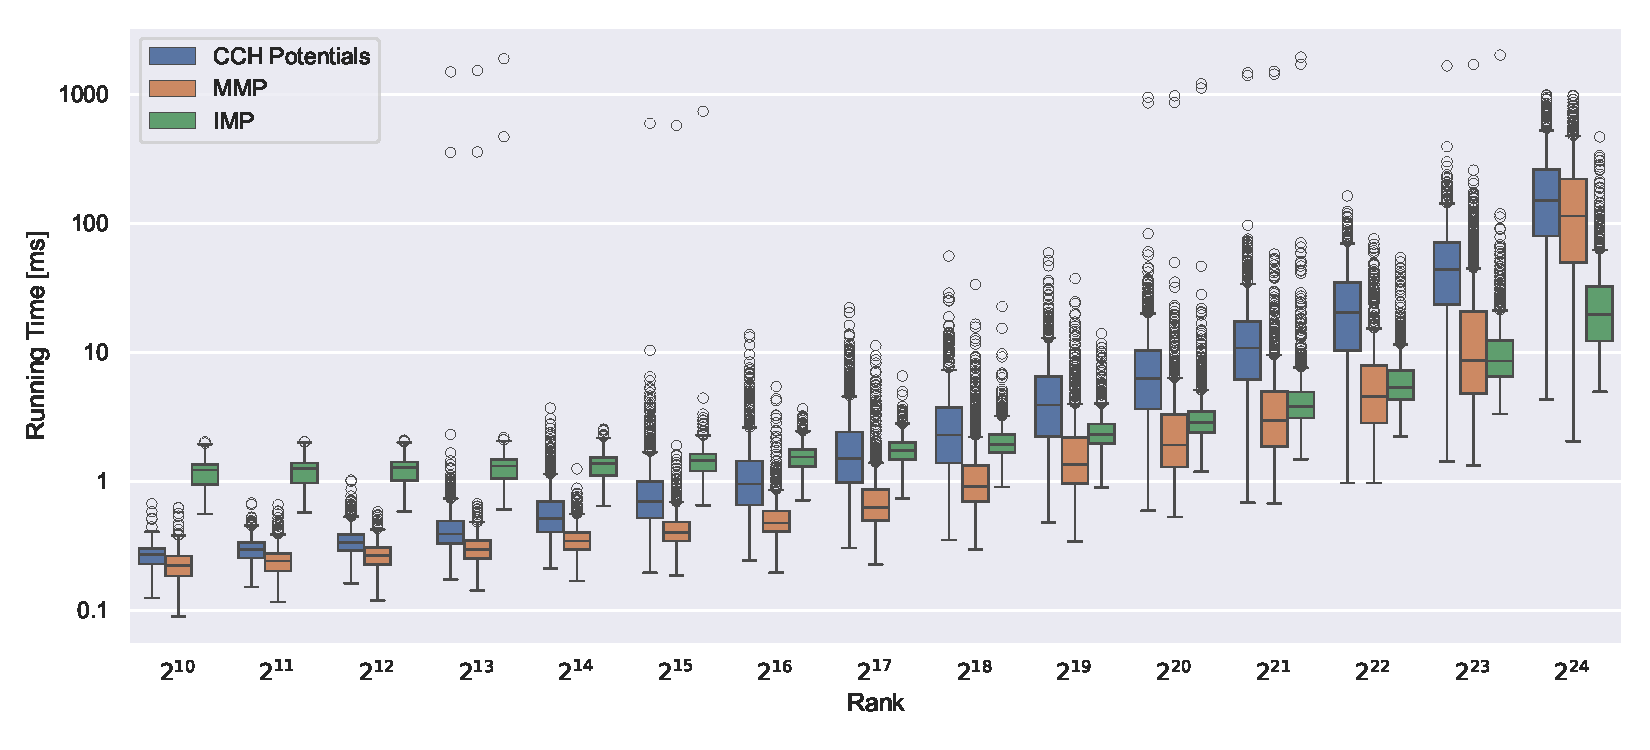
\includegraphics[width=\linewidth]{fig/ranks.pdf}
\caption{
TODO
The boxes cover the range between the first and third quartile.
The band in the box indicates the median, the whiskers cover 1.5 times the interquartile range.
All other running times are indicated as outliers.
}\label{fig:ranks}
\end{figure}

\begin{figure}
\centering
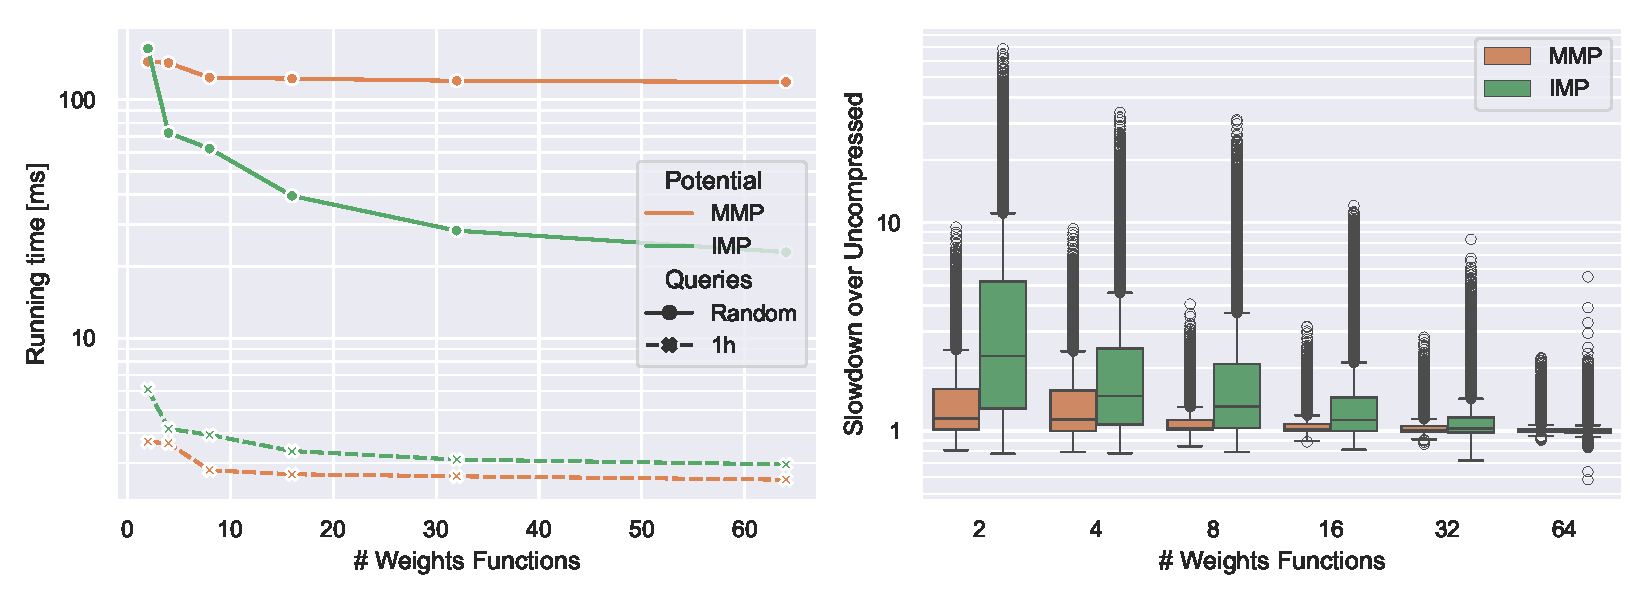
\includegraphics[width=\linewidth]{fig/compression.pdf}
\caption{
TODO
}\label{fig:compression}
\end{figure}

\section{Conclusion}

% \section{Typesetting instructions -- Summary}
% \label{sec:typesetting-summary}

% LIPIcs is a series of open access high-quality conference proceedings across all fields in informatics established in cooperation with Schloss Dagstuhl.
% In order to do justice to the high scientific quality of the conferences that publish their proceedings in the LIPIcs series, which is ensured by the thorough review process of the respective events, we believe that LIPIcs proceedings must have an attractive and consistent layout matching the standard of the series.
% Moreover, the quality of the metadata, the typesetting and the layout must also meet the requirements of other external parties such as indexing service, DOI registry, funding agencies, among others. The guidelines contained in this document serve as the baseline for the authors, editors, and the publisher to create documents that meet as many different requirements as possible.

% Please comply with the following instructions when preparing your article for a LIPIcs proceedings volume.
% \paragraph*{Minimum requirements}

% \begin{itemize}
% \item Use pdflatex and an up-to-date \LaTeX{} system.
% \item Use further \LaTeX{} packages and custom made macros carefully and only if required.
% \item Use the provided sectioning macros: \verb+\section+, \verb+\subsection+, \verb+\subsubsection+, \linebreak \verb+\paragraph+, \verb+\paragraph*+, and \verb+\subparagraph*+.
% \item Provide suitable graphics of at least 300dpi (preferably in PDF format).
% \item Use BibTeX and keep the standard style (\verb+plainurl+) for the bibliography.
% \item Please try to keep the warnings log as small as possible. Avoid overfull \verb+\hboxes+ and any kind of warnings/errors with the referenced BibTeX entries.
% \item Use a spellchecker to correct typos.
% \end{itemize}

% \paragraph*{Mandatory metadata macros}
% Please set the values of the metadata macros carefully since the information parsed from these macros will be passed to publication servers, catalogues and search engines.
% Avoid placing macros inside the metadata macros. The following metadata macros/environments are mandatory:
% \begin{itemize}
% \item \verb+\title+ and, in case of long titles, \verb+\titlerunning+.
% \item \verb+\author+, one for each author, even if two or more authors have the same affiliation.
% \item \verb+\authorrunning+ and \verb+\Copyright+ (concatenated author names)\\
% The \verb+\author+ macros and the \verb+\Copyright+ macro should contain full author names (especially with regard to the first name), while \verb+\authorrunning+ should contain abbreviated first names.
% \item \verb+\ccsdesc+ (ACM classification, see \url{https://www.acm.org/publications/class-2012}).
% \item \verb+\keywords+ (a comma-separated list of keywords).
% \item \verb+\relatedversion+ (if there is a related version, typically the ``full version''); please make sure to provide a persistent URL, e.\,g., at arXiv.
% \item \verb+\begin{abstract}...\end{abstract}+ .
% \end{itemize}

% \paragraph*{Please do not \ldots} %Do not override the \texttt{\seriesstyle}-defaults}
% Generally speaking, please do not override the \texttt{lipics-v2021}-style defaults. To be more specific, a short checklist also used by Dagstuhl Publishing during the final typesetting is given below.
% In case of \textbf{non-compliance} with these rules Dagstuhl Publishing will remove the corresponding parts of \LaTeX{} code and \textbf{replace it with the \texttt{lipics-v2021} defaults}. In serious cases, we may reject the LaTeX-source and expect the corresponding author to revise the relevant parts.
% \begin{itemize}
% \item Do not use a different main font. (For example, the \texttt{times} package is forbidden.)
% \item Do not alter the spacing of the \texttt{lipics-v2021.cls} style file.
% \item Do not use \verb+enumitem+ and \verb+paralist+. (The \texttt{enumerate} package is preloaded, so you can use
%  \verb+\begin{enumerate}[(a)]+ or the like.)
% \item Do not use ``self-made'' sectioning commands (e.\,g., \verb+\noindent{\bf My+ \verb+Paragraph}+).
% \item Do not hide large text blocks using comments or \verb+\iffalse+ $\ldots$ \verb+\fi+ constructions.
% \item Do not use conditional structures to include/exclude content. Instead, please provide only the content that should be published -- in one file -- and nothing else.
% \item Do not wrap figures and tables with text. In particular, the package \texttt{wrapfig} is not supported.
% \item Do not change the bibliography style. In particular, do not use author-year citations. (The
% \texttt{natbib} package is not supported.)
% \end{itemize}

% \enlargethispage{\baselineskip}

% This is only a summary containing the most relevant details. Please read the complete document ``LIPIcs: Instructions for Authors and the \texttt{lipics-v2021} Class'' for all details and don't hesitate to contact Dagstuhl Publishing (\url{mailto:publishing@dagstuhl.de}) in case of questions or comments:
% \href{http://drops.dagstuhl.de/styles/lipics-v2021/lipics-v2021-authors/lipics-v2021-authors-guidelines.pdf}{\texttt{http://drops.dagstuhl.de/styles/lipics-v2021/\newline lipics-v2021-authors/lipics-v2021-authors-guidelines.pdf}}

% \section{Lorem ipsum dolor sit amet}

% Lorem ipsum dolor sit amet, consectetur adipiscing elit \cite{DBLP:journals/cacm/Knuth74}. Praesent convallis orci arcu, eu mollis dolor. Aliquam eleifend suscipit lacinia. Maecenas quam mi, porta ut lacinia sed, convallis ac dui. Lorem ipsum dolor sit amet, consectetur adipiscing elit. Suspendisse potenti. Donec eget odio et magna ullamcorper vehicula ut vitae libero. Maecenas lectus nulla, auctor nec varius ac, ultricies et turpis. Pellentesque id ante erat. In hac habitasse platea dictumst. Curabitur a scelerisque odio. Pellentesque elit risus, posuere quis elementum at, pellentesque ut diam. Quisque aliquam libero id mi imperdiet quis convallis turpis eleifend.

% \begin{lemma}[Lorem ipsum]
% \label{lemma:lorem}
% Vestibulum sodales dolor et dui cursus iaculis. Nullam ullamcorper purus vel turpis lobortis eu tempus lorem semper. Proin facilisis gravida rutrum. Etiam sed sollicitudin lorem. Proin pellentesque risus at elit hendrerit pharetra. Integer at turpis varius libero rhoncus fermentum vitae vitae metus.
% \end{lemma}

% \begin{proof}
% Cras purus lorem, pulvinar et fermentum sagittis, suscipit quis magna.


% \proofsubparagraph*{Just some paragraph within the proof.}
% Nam liber tempor cum soluta nobis eleifend option congue nihil imperdiet doming id quod mazim placerat facer possim assum. Lorem ipsum dolor sit amet, consectetuer adipiscing elit, sed diam nonummy nibh euismod tincidunt ut laoreet dolore magna aliquam erat volutpat.
% \begin{claim}
% content...
% \end{claim}
% \begin{claimproof}
% content...
%     \begin{enumerate}
%         \item abc abc abc \claimqedhere{}
%     \end{enumerate}
% \end{claimproof}

% \end{proof}

% \begin{corollary}[Curabitur pulvinar, \cite{DBLP:books/mk/GrayR93}]
% \label{lemma:curabitur}
% Nam liber tempor cum soluta nobis eleifend option congue nihil imperdiet doming id quod mazim placerat facer possim assum. Lorem ipsum dolor sit amet, consectetuer adipiscing elit, sed diam nonummy nibh euismod tincidunt ut laoreet dolore magna aliquam erat volutpat.
% \end{corollary}

% \begin{proposition}\label{prop1}
% This is a proposition
% \end{proposition}

% \autoref{prop1} and \cref{prop1} \ldots

% \subsection{Curabitur dictum felis id sapien}

% Curabitur dictum \cref{lemma:curabitur} felis id sapien \autoref{lemma:curabitur} mollis ut venenatis tortor feugiat. Curabitur sed velit diam. Integer aliquam, nunc ac egestas lacinia, nibh est vehicula nibh, ac auctor velit tellus non arcu. Vestibulum lacinia ipsum vitae nisi ultrices eget gravida turpis laoreet. Duis rutrum dapibus ornare. Nulla vehicula vulputate iaculis. Proin a consequat neque. Donec ut rutrum urna. Morbi scelerisque turpis sed elit sagittis eu scelerisque quam condimentum. Pellentesque habitant morbi tristique senectus et netus et malesuada fames ac turpis egestas. Aenean nec faucibus leo. Cras ut nisl odio, non tincidunt lorem. Integer purus ligula, venenatis et convallis lacinia, scelerisque at erat. Fusce risus libero, convallis at fermentum in, dignissim sed sem. Ut dapibus orci vitae nisl viverra nec adipiscing tortor condimentum \cite{DBLP:journals/cacm/Dijkstra68a}. Donec non suscipit lorem. Nam sit amet enim vitae nisl accumsan pretium.

% \begin{lstlisting}[caption={Useless code.},label=list:8-6,captionpos=t,float,abovecaptionskip=-\medskipamount]
% for i:=maxint to 0 do
% begin
%     j:=square(root(i));
% end;
% \end{lstlisting}

% \subsection{Proin ac fermentum augue}

% Proin ac fermentum augue. Nullam bibendum enim sollicitudin tellus egestas lacinia euismod orci mollis. Nulla facilisi. Vivamus volutpat venenatis sapien, vitae feugiat arcu fringilla ac. Mauris sapien tortor, sagittis eget auctor at, vulputate pharetra magna. Sed congue, dui nec vulputate convallis, sem nunc adipiscing dui, vel venenatis mauris sem in dui. Praesent a pretium quam. Mauris non mauris sit amet eros rutrum aliquam id ut sapien. Nulla aliquet fringilla sagittis. Pellentesque eu metus posuere nunc tincidunt dignissim in tempor dolor. Nulla cursus aliquet enim. Cras sapien risus, accumsan eu cursus ut, commodo vel velit. Praesent aliquet consectetur ligula, vitae iaculis ligula interdum vel. Integer faucibus faucibus felis.

% \begin{itemize}
% \item Ut vitae diam augue.
% \item Integer lacus ante, pellentesque sed sollicitudin et, pulvinar adipiscing sem.
% \item Maecenas facilisis, leo quis tincidunt egestas, magna ipsum condimentum orci, vitae facilisis nibh turpis et elit.
% \end{itemize}

% \begin{remark}
% content...
% \end{remark}

% \section{Pellentesque quis tortor}

% Nec urna malesuada sollicitudin. Nulla facilisi. Vivamus aliquam tempus ligula eget ornare. Praesent eget magna ut turpis mattis cursus. Aliquam vel condimentum orci. Nunc congue, libero in gravida convallis \cite{DBLP:conf/focs/HopcroftPV75}, orci nibh sodales quam, id egestas felis mi nec nisi. Suspendisse tincidunt, est ac vestibulum posuere, justo odio bibendum urna, rutrum bibendum dolor sem nec tellus.

% \begin{lemma} [Quisque blandit tempus nunc]
% Sed interdum nisl pretium non. Mauris sodales consequat risus vel consectetur. Aliquam erat volutpat. Nunc sed sapien ligula. Proin faucibus sapien luctus nisl feugiat convallis faucibus elit cursus. Nunc vestibulum nunc ac massa pretium pharetra. Nulla facilisis turpis id augue venenatis blandit. Cum sociis natoque penatibus et magnis dis parturient montes, nascetur ridiculus mus.
% \end{lemma}

% Fusce eu leo nisi. Cras eget orci neque, eleifend dapibus felis. Duis et leo dui. Nam vulputate, velit et laoreet porttitor, quam arcu facilisis dui, sed malesuada risus massa sit amet neque.

% \section{Morbi eros magna}

% Morbi eros magna, vestibulum non posuere non, porta eu quam. Maecenas vitae orci risus, eget imperdiet mauris. Donec massa mauris, pellentesque vel lobortis eu, molestie ac turpis. Sed condimentum convallis dolor, a dignissim est ultrices eu. Donec consectetur volutpat eros, et ornare dui ultricies id. Vivamus eu augue eget dolor euismod ultrices et sit amet nisi. Vivamus malesuada leo ac leo ullamcorper tempor. Donec justo mi, tempor vitae aliquet non, faucibus eu lacus. Donec dictum gravida neque, non porta turpis imperdiet eget. Curabitur quis euismod ligula.


%%
%% Bibliography
%%

%% Please use bibtex, 

\bibliography{references}

\appendix

\section{Time-Dependent A* Potentials and Correctness Properties}\label{sec:correctness}

In this section, we analyze correctness properties for time-dependent A* potentials.
For the analysis, it is oftentimes more practical the use arrival time functions instead of travel time functions.
Given a travel time function $w$, we denote the respective arrival time function as $\hat{w}(uv, \tau) := w(uv, \tau) + \tau$.
With arrival time functions, we can represent path lengths simply as the composition of the edges arrival time functions.
Similarly to the time-independent case, we can define a modified weight function $w'$ such that running A* on a graph $G$ with time-dependent travel times $w$ with a time-dependent potential $\pi_t$ is equivalent to running Dijkstra's on the same graph with modified weights $w'$.
Consider a vertex $u$ with an arrival time of $\tau$.
In A*, its queue key is $\tau' = \hat{\pi}_t(u, \tau)$.
When relaxing an edge $uv$, we get a queue key of $\hat{\pi}_t(u, \hat{w}(uv, \tau))$ at $v$.
Thus, by definition we get $\hat{w}'(uv, \tau') = \hat{\pi}_t(v, \hat{w}(uv, \hat{\pi}_t(u)^{-1}(\tau')))$ where $\hat{\pi}_t(u)^{-1}$ is the inverted arrival time function, i.e.\ a \emph{departure time} function.
For $\hat{\pi}_t(u)^{-1}$ to be well defined, we need $\tau_1 \neq \tau_2 \implies \hat{\pi}_t(\tau_1) \neq \hat{\pi}_t(\tau_2)$.
Therefore, for potentials we require the \emph{strong First-In First-Out} property:
\[
\pi_t(v, \tau) < \pi_t(v, \tau + \epsilon) + \epsilon, v \in V, \tau \in T, \epsilon \geq 0
\]
Note that potentials which only adhere to the regular FIFO property in practice likely work just as well.
It just breaks the well-definedness of the modified weights for an theoretically equivalent run of Dijkstra's algorithm.

Shortest paths for these modified weights are the same es with the original weights.
Consider the weights of two different $s$-$t$ paths.
The initial potential at $s$ is the same for both paths, all the inner potential evaluations cancel out and the potentials at $s$ and the final potential evaluation at $t$ cannot change the order due to the FIFO property.

We can follow that when these modified weights do not have any negative travel times, then Dijkstra and thus A* will obtain correct result. % running time
This leads to the \emph{feasibility} property for time-dependent potentials:
\[
\hat{w}'(uv, \tau') = \hat{\pi}_t(v, \hat{w}(uv, \hat{\pi}_t(u)^{-1}(\tau'))) \geq \tau'
\]
To simplify correctness proofs for potentials, we reform this to a simpler equivalent property:
\begin{align*}
\hat{\pi}_t(v, \hat{w}(uv, \tau)) & \geq \hat{\pi}_t(u, \tau) \\
\pi_t(v, w(uv, \tau) + \tau) + w(uv, \tau) + \tau & \geq \pi_t(u, \tau) + \tau \\
\pi_t(v, w(uv, \tau) + \tau) + w(uv, \tau) - \pi_t(u, \tau) & \geq 0
\end{align*}
This formulation also shows that the time-dependent feasibility is a generalization to the classical feasibility property.

The third property is the \emph{lower bound} property:
\[
\pi_t(v, \tau) \leq \dist(v,t,\tau)
\]
With a potential fulfilling this property, A* will have found the shortest path once the target vertex was settled, even if the potential is not feasible.
This is because every shortest path vertex must have a queue key smaller than the target and by induction all these vertexes must have been settled before the target.
Also, even with negative travel times, negative cycles are not possible.
Consider a cycle $C$ starting and ending at vertex $v$.
The length of the cycle with the modified weights is $w'(C, \tau') = \hat{\pi}_t(v, \hat(w)(C, \hat{\pi}_t(u)^{-1}(\tau')))$ because all inner potential functions cancel out.
As $\hat{\pi}_t(v)$ has to adhere to the FIFO property, the length of $C$ cannot be negative.
Thus, A* with lower bound potentials will obtain correct results.
However, the running time may be exponential in the graph size.

Crucially, to guarantee correctness it is not necessary to adhere to these properties for all $\tau$.
Assume we are running A* to answer a query from $s$ to $t$ with departure $\tdep$.
Clearly, A* will never invoke the potential of vertex $v$ with $\tau < \dist(s,v,\tdep)$.
Therefore, it is sufficient to guarantee the strong FIFO property at vertex $v$ and the feasibility property for edge $vw$ for $\tau \geq \dist(s,v,\tdep)$.
For the lower bound property it even suffices to guarantee it only at exactly $\tau = \dist(s,v,\tdep)$.

\subsection{Multi-Metric Potential Correctness}

For any given single query, the multi metric potential actually is a time-independent potential which returns exact shortest distance with respect to a valid lower bound weight function.
Constant potentials trivially adhere to the strong FIFO property.
Also, as shown in~\cite{strasser_et_al:LIPIcs.SEA.2021.6}, shortest distances by a lower bound weight function are a feasible potential.
% metric switching?

\subsection{Interval-Minimum Potential Correctness}

The Interval-Minimum Potential is not feasible because we use piecewise constant functions for the the shortcut travel time lower bounds.
Still, it does satisfy the strong FIFO property because for any given single query, the estimates are constant.
Moreover, the estimates are lower bounds on the distances.
This directly follows from the correctness of the CATCHUp preprocessing and the Lazy RPHAST algorithm.
% metric switching?

% \section{Styles of lists, enumerations, and descriptions}\label{sec:itemStyles}

% List of different predefined enumeration styles:

% \begin{itemize}
% \item \verb|\begin{itemize}...\end{itemize}|
% \item \dots
% \item \dots
% %\item \dots
% \end{itemize}

% \begin{enumerate}
% \item \verb|\begin{enumerate}...\end{enumerate}|
% \item \dots
% \item \dots
% %\item \dots
% \end{enumerate}

% \begin{alphaenumerate}
% \item \verb|\begin{alphaenumerate}...\end{alphaenumerate}|
% \item \dots
% \item \dots
% %\item \dots
% \end{alphaenumerate}

% \begin{romanenumerate}
% \item \verb|\begin{romanenumerate}...\end{romanenumerate}|
% \item \dots
% \item \dots
% %\item \dots
% \end{romanenumerate}

% \begin{bracketenumerate}
% \item \verb|\begin{bracketenumerate}...\end{bracketenumerate}|
% \item \dots
% \item \dots
% %\item \dots
% \end{bracketenumerate}

% \begin{description}
% \item[Description 1] \verb|\begin{description} \item[Description 1]  ...\end{description}|
% \item[Description 2] Fusce eu leo nisi. Cras eget orci neque, eleifend dapibus felis. Duis et leo dui. Nam vulputate, velit et laoreet porttitor, quam arcu facilisis dui, sed malesuada risus massa sit amet neque.
% \item[Description 3]  \dots
% %\item \dots
% \end{description}

% \cref{testenv-proposition} and \autoref{testenv-proposition} ...

% \section{Theorem-like environments}\label{sec:theorem-environments}

% List of different predefined enumeration styles:

% \begin{theorem}\label{testenv-theorem}
% Fusce eu leo nisi. Cras eget orci neque, eleifend dapibus felis. Duis et leo dui. Nam vulputate, velit et laoreet porttitor, quam arcu facilisis dui, sed malesuada risus massa sit amet neque.
% \end{theorem}

% \begin{lemma}\label{testenv-lemma}
% Fusce eu leo nisi. Cras eget orci neque, eleifend dapibus felis. Duis et leo dui. Nam vulputate, velit et laoreet porttitor, quam arcu facilisis dui, sed malesuada risus massa sit amet neque.
% \end{lemma}

% \begin{corollary}\label{testenv-corollary}
% Fusce eu leo nisi. Cras eget orci neque, eleifend dapibus felis. Duis et leo dui. Nam vulputate, velit et laoreet porttitor, quam arcu facilisis dui, sed malesuada risus massa sit amet neque.
% \end{corollary}

% \begin{proposition}\label{testenv-proposition}
% Fusce eu leo nisi. Cras eget orci neque, eleifend dapibus felis. Duis et leo dui. Nam vulputate, velit et laoreet porttitor, quam arcu facilisis dui, sed malesuada risus massa sit amet neque.
% \end{proposition}

% \begin{conjecture}\label{testenv-conjecture}
% Fusce eu leo nisi. Cras eget orci neque, eleifend dapibus felis. Duis et leo dui. Nam vulputate, velit et laoreet porttitor, quam arcu facilisis dui, sed malesuada risus massa sit amet neque.
% \end{conjecture}

% \begin{observation}\label{testenv-observation}
% Fusce eu leo nisi. Cras eget orci neque, eleifend dapibus felis. Duis et leo dui. Nam vulputate, velit et laoreet porttitor, quam arcu facilisis dui, sed malesuada risus massa sit amet neque.
% \end{observation}

% \begin{exercise}\label{testenv-exercise}
% Fusce eu leo nisi. Cras eget orci neque, eleifend dapibus felis. Duis et leo dui. Nam vulputate, velit et laoreet porttitor, quam arcu facilisis dui, sed malesuada risus massa sit amet neque.
% \end{exercise}

% \begin{definition}\label{testenv-definition}
% Fusce eu leo nisi. Cras eget orci neque, eleifend dapibus felis. Duis et leo dui. Nam vulputate, velit et laoreet porttitor, quam arcu facilisis dui, sed malesuada risus massa sit amet neque.
% \end{definition}

% \begin{example}\label{testenv-example}
% Fusce eu leo nisi. Cras eget orci neque, eleifend dapibus felis. Duis et leo dui. Nam vulputate, velit et laoreet porttitor, quam arcu facilisis dui, sed malesuada risus massa sit amet neque.
% \end{example}

% \begin{note}\label{testenv-note}
% Fusce eu leo nisi. Cras eget orci neque, eleifend dapibus felis. Duis et leo dui. Nam vulputate, velit et laoreet porttitor, quam arcu facilisis dui, sed malesuada risus massa sit amet neque.
% \end{note}

% \begin{note*}
% Fusce eu leo nisi. Cras eget orci neque, eleifend dapibus felis. Duis et leo dui. Nam vulputate, velit et laoreet porttitor, quam arcu facilisis dui, sed malesuada risus massa sit amet neque.
% \end{note*}

% \begin{remark}\label{testenv-remark}
% Fusce eu leo nisi. Cras eget orci neque, eleifend dapibus felis. Duis et leo dui. Nam vulputate, velit et laoreet porttitor, quam arcu facilisis dui, sed malesuada risus massa sit amet neque.
% \end{remark}

% \begin{remark*}
% Fusce eu leo nisi. Cras eget orci neque, eleifend dapibus felis. Duis et leo dui. Nam vulputate, velit et laoreet porttitor, quam arcu facilisis dui, sed malesuada risus massa sit amet neque.
% \end{remark*}

% \begin{claim}\label{testenv-claim}
% Fusce eu leo nisi. Cras eget orci neque, eleifend dapibus felis. Duis et leo dui. Nam vulputate, velit et laoreet porttitor, quam arcu facilisis dui, sed malesuada risus massa sit amet neque.
% \end{claim}

% \begin{claim*}\label{testenv-claim2}
% Fusce eu leo nisi. Cras eget orci neque, eleifend dapibus felis. Duis et leo dui. Nam vulputate, velit et laoreet porttitor, quam arcu facilisis dui, sed malesuada risus massa sit amet neque.
% \end{claim*}

% \begin{proof}
% Fusce eu leo nisi. Cras eget orci neque, eleifend dapibus felis. Duis et leo dui. Nam vulputate, velit et laoreet porttitor, quam arcu facilisis dui, sed malesuada risus massa sit amet neque.
% \end{proof}

% \begin{claimproof}
% Fusce eu leo nisi. Cras eget orci neque, eleifend dapibus felis. Duis et leo dui. Nam vulputate, velit et laoreet porttitor, quam arcu facilisis dui, sed malesuada risus massa sit amet neque.
% \end{claimproof}

\end{document}
